\documentclass[11pt,a4paper]{article}

% ── Packages ──────────────────────────────────────────
\usepackage[margin=1in]{geometry}
\usepackage{graphicx}
\usepackage{booktabs}
\usepackage{hyperref}
\usepackage{listings}
\usepackage{xcolor}
\usepackage{float}
\usepackage{enumitem}
\usepackage{amsmath}
\usepackage{caption}
\usepackage{subcaption}
\usepackage{fancyhdr}

% ── Colors ────────────────────────────────────────────
\definecolor{codeblue}{RGB}{0,102,204}
\definecolor{codegray}{RGB}{100,100,100}
\definecolor{codebg}{RGB}{245,245,245}

% ── Listings ──────────────────────────────────────────
\lstset{
  basicstyle=\ttfamily\small,
  backgroundcolor=\color{codebg},
  keywordstyle=\color{codeblue}\bfseries,
  commentstyle=\color{codegray},
  breaklines=true,
  frame=single,
  rulecolor=\color{codegray!30},
  numbers=none,
  xleftmargin=6pt,
  xrightmargin=6pt,
  aboveskip=8pt,
  belowskip=8pt,
}

% ── Header / Footer ──────────────────────────────────
\pagestyle{fancy}
\fancyhf{}
\rhead{CS242 -- Spring 2026}
\lhead{Group 7: TMDB Movie Search Engine}
\rfoot{Page \thepage}

% ── Title ─────────────────────────────────────────────
\title{
  \textbf{CS242 Part B Report} \\[6pt]
  \Large TMDB Movie Search Engine: \\
  Dual-Index Retrieval with Elasticsearch and BERT
}
\author{
  Group 7 --- UC Riverside \\[4pt]
  % ── TODO: Replace with actual names ──
  \textit{Member 1 Name, Member 2 Name, Member 3 Name}
}
\date{Spring 2026}

\begin{document}
\maketitle
\thispagestyle{fancy}

% ══════════════════════════════════════════════════════
\section{Collaboration Details}
% ══════════════════════════════════════════════════════

% ── TODO: Fill in actual names and contributions ──
\begin{table}[H]
\centering
\begin{tabular}{@{}lp{10cm}@{}}
\toprule
\textbf{Member} & \textbf{Contribution} \\
\midrule
Member 1 & TODO: Describe contribution \\
Member 2 & TODO: Describe contribution \\
Member 3 & TODO: Describe contribution \\
\bottomrule
\end{tabular}
\caption{Team member contributions.}
\end{table}

% ══════════════════════════════════════════════════════
\section{System Overview}
% ══════════════════════════════════════════════════════

\subsection{Architecture}

The system consists of four components built across Parts A1, A2, B1, and B2:

\begin{enumerate}[nosep]
  \item \textbf{Scrapy Crawler (Part A1)} --- Two-phase crawling pipeline that collects 221,645 movie records (1.09\,GB) from the TMDB API.
  \item \textbf{Elasticsearch Index (Part A2)} --- Sparse (BM25) index with custom English analyzers for keyword-based retrieval.
  \item \textbf{BERT + FAISS Index (Part B1)} --- Dense semantic index using Sentence-BERT embeddings and FAISS for meaning-based retrieval.
  \item \textbf{Flask Web Application (Part B2)} --- Unified search interface supporting dual-index querying, side-by-side comparison, and a world map visualization.
\end{enumerate}

\noindent The overall data flow is:

\begin{lstlisting}
TMDB API --> Scrapy Crawler --> 221,645 JSON files (data/movies/)
  --> Elasticsearch Indexer --> ES BM25 Index
  --> BERT Notebook (Colab) --> FAISS Index + Metadata
  --> Flask Web App --> User Query --> Both Indexes --> Ranked Results
\end{lstlisting}

\begin{figure}[H]
\centering
% ── TODO: Insert architecture diagram ──
\fbox{\parbox{0.85\textwidth}{\centering\vspace{3cm}
\textit{TODO: Insert system architecture diagram here.}
\vspace{3cm}}}
\caption{System architecture overview.}
\label{fig:architecture}
\end{figure}

% ──────────────────────────────────────────────────────
\subsection{BERT Index: Model Choice and Indexing Schema}
\label{sec:bert}
% ──────────────────────────────────────────────────────

\subsubsection{Model Choice}

We use \texttt{sentence-transformers/all-MiniLM-L6-v2}, a distilled Sentence-BERT model with the following properties:

\begin{table}[H]
\centering
\begin{tabular}{@{}ll@{}}
\toprule
\textbf{Property} & \textbf{Value} \\
\midrule
Architecture & 6-layer Transformer (distilled from BERT-base) \\
Output dimension & 384 \\
Max sequence length & 512 tokens \\
Training objective & Sentence similarity (contrastive learning) \\
Inference speed & $\sim$5$\times$ faster than \texttt{bert-base-uncased} \\
\bottomrule
\end{tabular}
\caption{BERT model properties.}
\end{table}

\noindent \textbf{Why this model?}
\begin{itemize}[nosep]
  \item It is \textit{fine-tuned for sentence similarity}, which directly aligns with our task of matching a query sentence to movie descriptions.
  \item The 384-dimensional output produces a compact index ($\sim$320\,MB for 220K vectors), roughly half the size of a 768-dim model.
  \item The 6-layer architecture is fast enough for real-time query encoding in the web application ($<$100\,ms per query on CPU).
\end{itemize}

\subsubsection{Indexing Schema}

For each movie, we construct a single text passage by combining key fields:

\begin{lstlisting}
Title: {title} {title} {title}
Overview: {overview}
Tagline: {tagline}
Genres: {genre names}
Cast: {top 5 actor names}
Director: {director names}
\end{lstlisting}

\noindent The title is repeated three times to increase its weight in the embedding. This passage is then processed as follows:

\begin{enumerate}[nosep]
  \item \textbf{Tokenization}: WordPiece tokenizer splits text into sub-word tokens, padded/truncated to 512 tokens.
  \item \textbf{Encoding}: The 6-layer Transformer produces a $[512 \times 384]$ tensor.
  \item \textbf{Mean Pooling}: All token vectors are averaged into a single 384-dimensional vector, weighted by the attention mask to ignore padding tokens.
  \item \textbf{FAISS Storage}: The vector is added to a \texttt{IndexFlatL2} index (exact brute-force L2 search with no approximation).
\end{enumerate}

\noindent The indexing is performed in batches of 64 on a Google Colab T4 GPU, processing all 220,015 movies in approximately 12 minutes.

A parallel metadata list (\texttt{movie\_metadata.pkl}) stores structured information (title, overview, genres, origin\_country, vote\_average, etc.) for each vector position, enabling result display without a secondary database lookup.

% ──────────────────────────────────────────────────────
\subsection{BERT Index Ranking}
\label{sec:bert-ranking}
% ──────────────────────────────────────────────────────

At query time, ranking proceeds as follows:

\begin{enumerate}[nosep]
  \item The user's query string is encoded by the same \texttt{all-MiniLM-L6-v2} model into a 384-dim vector using identical tokenization and mean-pooling.
  \item FAISS performs an exhaustive L2 (Euclidean distance) search across all 220,015 stored vectors and returns the \texttt{top\_k} nearest neighbors.
  \item Raw L2 distances are converted to similarity scores using:
  \[
    \text{similarity} = \frac{1}{1 + d_{\text{L2}}}
  \]
  where $d_{\text{L2}}$ is the L2 distance. Lower distance yields higher similarity, bounded in $(0, 1]$.
  \item If a country filter is active, FAISS over-fetches by $5\times$ and post-filters by \texttt{origin\_country} from the metadata.
  \item The metadata list is indexed by FAISS vector position to retrieve titles, overviews, genres, etc.\ for the result cards.
\end{enumerate}

\noindent Because \texttt{IndexFlatL2} performs exact (non-approximate) search, ranking is deterministic and exhaustive --- every movie in the corpus is compared against the query vector.

% ──────────────────────────────────────────────────────
\subsection{Elasticsearch (Lucene) Index and Query}
\label{sec:es}
% ──────────────────────────────────────────────────────

\subsubsection{Index Design}

The Elasticsearch index uses a custom analyzer named \texttt{en\_tmdb\_english\_stem}, which applies the following filter chain:

\begin{enumerate}[nosep]
  \item \texttt{lowercase} --- case normalization
  \item \texttt{asciifolding} --- Unicode $\to$ ASCII (e.g., \texttt{caf\'e} $\to$ \texttt{cafe})
  \item \texttt{english\_possessive\_stemmer} --- removes possessive suffixes (\texttt{'s})
  \item \texttt{english\_stop} --- removes English stop words
  \item \texttt{english\_stemmer} --- Porter stemming (e.g., \texttt{running} $\to$ \texttt{run})
\end{enumerate}

\noindent The index schema defines 25 fields organized into four categories:

\begin{table}[H]
\centering
\small
\begin{tabular}{@{}llp{7.5cm}@{}}
\toprule
\textbf{Category} & \textbf{Fields} & \textbf{Type \& Purpose} \\
\midrule
Full text & \texttt{title}, \texttt{overview}, \texttt{tagline}, \texttt{reviews\_text}, \texttt{all\_text} & \texttt{text} with custom analyzer; \texttt{all\_text} merges all text fields for fallback matching \\
People & \texttt{cast\_names}, \texttt{crew\_names}, \texttt{cast\_characters} & \texttt{text} with analyzer + \texttt{.raw} keyword sub-field \\
Filter/Facet & \texttt{genres}, \texttt{origin\_country}, \texttt{status}, \texttt{crew\_jobs} & \texttt{keyword} for exact-match filtering and aggregations \\
Numeric & \texttt{vote\_average}, \texttt{vote\_count}, \texttt{popularity}, \texttt{release\_year} & \texttt{float}/\texttt{integer} for sorting and range filters \\
\bottomrule
\end{tabular}
\caption{Elasticsearch field schema (selected fields).}
\end{table}

\subsubsection{Query Strategy}

The search module uses Elasticsearch's \texttt{multi\_match} query with the following configuration:

\begin{lstlisting}[language=Python]
"multi_match": {
    "query": user_query,
    "fields": [
        "title^3",            # 3x boost
        "original_title^2",   # 2x boost
        "overview^2",         # 2x boost
        "tagline^1.5",        # 1.5x boost
        "cast_names^1.5",     # 1.5x boost
        "crew_names",         # 1x (default)
        "all_text",           # 1x fallback
    ],
    "type": "best_fields",
    "fuzziness": "AUTO",
}
\end{lstlisting}

\noindent Key design decisions:

\begin{itemize}[nosep]
  \item \textbf{\texttt{best\_fields} type}: Scores each field independently and takes the highest-scoring field's score, rather than summing across all fields. This prevents a mediocre match in many fields from outranking a strong match in `title`.
  \item \textbf{Field boosting}: \texttt{title\^{}3} ensures that an exact title match ranks highest. \texttt{overview\^{}2} reflects that plot descriptions are the most semantically rich text field.
  \item \textbf{\texttt{fuzziness: AUTO}}: Allows edit-distance tolerance (1 edit for 3--5 char terms, 2 edits for 6+ char terms), improving recall for typos without sacrificing precision on short queries.
  \item \textbf{\texttt{all\_text} as fallback}: A combined field that merges title, overview, tagline, cast, crew, and reviews. If none of the boosted fields match, \texttt{all\_text} provides baseline recall.
  \item \textbf{Country filtering}: Implemented as a \texttt{bool.filter} with a \texttt{term} query on the \texttt{origin\_country} keyword field, enabling post-filter via the world map without affecting relevance scoring.
\end{itemize}

\noindent Elasticsearch's underlying Lucene engine scores documents using BM25 (Best Matching 25), which considers term frequency, inverse document frequency, and document length normalization.

% ──────────────────────────────────────────────────────
\subsection{Index Construction Runtime}
\label{sec:runtime}
% ──────────────────────────────────────────────────────

\begin{table}[H]
\centering
\begin{tabular}{@{}lrrll@{}}
\toprule
\textbf{Index Type} & \textbf{Documents} & \textbf{Runtime (s)} & \textbf{Throughput} & \textbf{Hardware} \\
\midrule
BERT + FAISS & 220,015 & 722.34 & 304.8 docs/s & Google Colab T4 GPU \\
Elasticsearch (BM25) & 220,015 & 1,333.05 & 165.0 docs/s & Server CPU \\
\bottomrule
\end{tabular}
\caption{Index construction runtime comparison.}
\label{tab:runtime}
\end{table}

\noindent The Elasticsearch index for scalability benchmarking was also profiled at incremental corpus sizes:

\begin{table}[H]
\centering
\begin{tabular}{@{}rrr@{}}
\toprule
\textbf{Documents} & \textbf{Runtime (s)} & \textbf{Throughput (docs/s)} \\
\midrule
10,000 & 5.34 & 1,872.66 \\
50,000 & 11.27 & 4,436.56 \\
100,000 & 20.59 & 4,856.73 \\
150,000 & 30.58 & 4,905.17 \\
220,243 & 42.93 & 5,130.28 \\
\bottomrule
\end{tabular}
\caption{Elasticsearch indexing runtime at incremental corpus sizes (benchmark run).}
\label{tab:es-benchmark}
\end{table}

\begin{figure}[H]
\centering
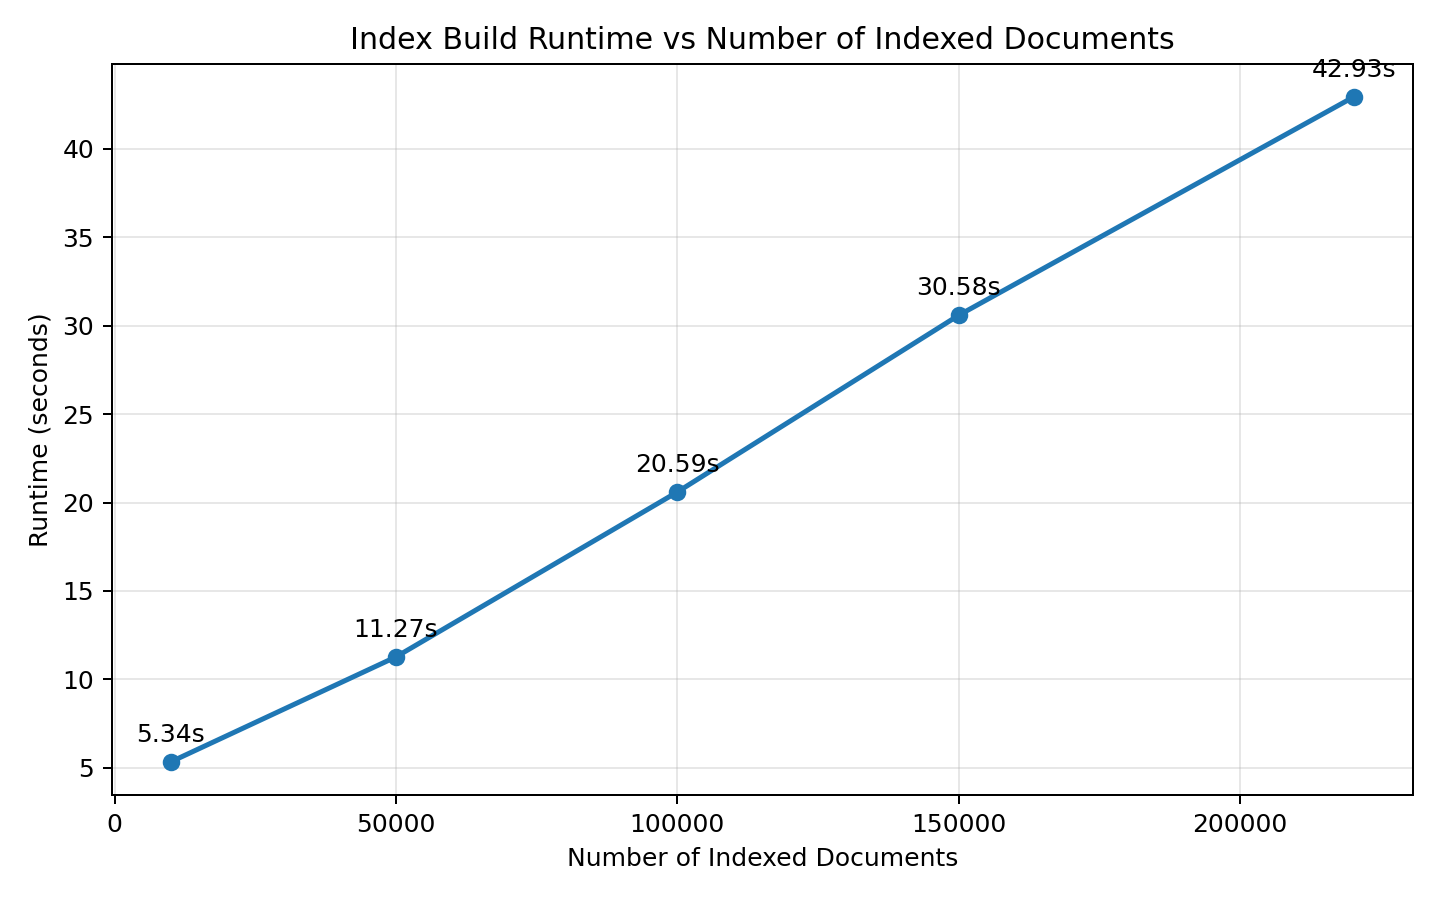
\includegraphics[width=0.75\textwidth]{../a2_index/benchmarks/runtime_plot.png}
\caption{Elasticsearch index build runtime vs.\ number of documents. Runtime scales approximately linearly; throughput stabilizes above $\sim$4,800 docs/s after warm-up.}
\label{fig:runtime-plot}
\end{figure}

\subsubsection{Runtime Discussion}

\textbf{BERT is faster in total time (722\,s vs.\ 1,333\,s).} This is counterintuitive at first glance, since BERT involves neural network inference while ES performs simpler text tokenization and inverted index construction. The explanation lies in the hardware and workload differences:

\begin{itemize}[nosep]
  \item \textbf{GPU parallelism}: BERT encoding runs on a T4 GPU with 2,560 CUDA cores, processing batches of 64 documents simultaneously through the neural network. This massive parallelism offsets the per-document computational cost.
  \item \textbf{FAISS writes are trivial}: Adding a 384-float vector to \texttt{IndexFlatL2} is a simple array append ($O(1)$ amortized), whereas ES must tokenize text, compute term statistics, update inverted index postings, and manage segment merges.
  \item \textbf{ES I/O overhead}: Elasticsearch writes to disk with translog durability guarantees. Each bulk chunk involves network serialization, JSON parsing, Lucene segment writes, and periodic segment merges --- all CPU-bound operations.
  \item \textbf{Different bottlenecks}: BERT's bottleneck is compute (matrix multiplications on GPU); ES's bottleneck is I/O and text processing (on CPU). The GPU's throughput advantage outweighs the per-document complexity of BERT inference.
\end{itemize}

\noindent \textbf{Note}: The comparison reflects real project conditions (Colab GPU for BERT vs.\ server/local CPU for ES) rather than a hardware-controlled benchmark. On identical hardware without GPU, BERT indexing would be significantly slower.

% ──────────────────────────────────────────────────────
\subsection{Ranking Quality Comparison: Elasticsearch vs.\ BERT}
\label{sec:comparison}
% ──────────────────────────────────────────────────────

The web application's \textbf{Compare} tab allows running the same query on both indexes simultaneously. Below we present representative examples.

\subsubsection{Example 1: ``funny space adventure'' (BERT wins)}

\begin{table}[H]
\centering
\small
\begin{tabular}{@{}clcl@{}}
\toprule
\textbf{Rank} & \textbf{Elasticsearch} & \textbf{Rank} & \textbf{BERT + FAISS} \\
\midrule
1 & Space Adventure Cobra & 1 & Guardians of the Galaxy \\
2 & The Adventures of Tintin & 2 & Galaxy Quest \\
3 & Space Buddies & 3 & Spaceballs \\
4 & Adventures in Space and Time & 4 & Mars Attacks! \\
5 & Space Chimps & 5 & The Hitchhiker's Guide to the Galaxy \\
\bottomrule
\end{tabular}
\caption{Query: ``funny space adventure'' --- BERT captures the \textit{semantic} meaning (comedy + space), while ES matches individual keywords.}
\label{tab:compare1}
\end{table}

\noindent \textbf{Analysis}: Elasticsearch matches the literal words ``space'' and ``adventure'' independently, returning results that contain these terms regardless of comedic content. BERT understands that ``funny space adventure'' implies a \textit{comedy set in space}, producing results like \textit{Guardians of the Galaxy} and \textit{Spaceballs} that are semantically aligned.

\subsubsection{Example 2: ``Brad Pitt'' (Elasticsearch wins)}

\begin{table}[H]
\centering
\small
\begin{tabular}{@{}clcl@{}}
\toprule
\textbf{Rank} & \textbf{Elasticsearch} & \textbf{Rank} & \textbf{BERT + FAISS} \\
\midrule
1 & Fight Club & 1 & Fight Club \\
2 & Troy & 2 & Bullet Train \\
3 & Once Upon a Time in Hollywood & 3 & Troy \\
4 & Se7en & 4 & The Lost City of Z \\
5 & The Big Short & 5 & Once Upon a Time in Hollywood \\
\bottomrule
\end{tabular}
\caption{Query: ``Brad Pitt'' --- ES leverages exact keyword matching on \texttt{cast\_names\^{}1.5} with high precision.}
\label{tab:compare2}
\end{table}

\noindent \textbf{Analysis}: For entity name queries, Elasticsearch excels because \texttt{cast\_names} is a dedicated boosted field and BM25's exact term matching is ideal for proper nouns. BERT, which encodes ``Brad Pitt'' as a semantic vector, may surface movies whose \textit{descriptions} are similar to the concept of Brad Pitt rather than movies that literally star him.

\subsubsection{Example 3: ``a movie about dreams within dreams'' (BERT wins)}

\begin{table}[H]
\centering
\small
\begin{tabular}{@{}clcl@{}}
\toprule
\textbf{Rank} & \textbf{Elasticsearch} & \textbf{Rank} & \textbf{BERT + FAISS} \\
\midrule
1 & Dreams & 1 & Inception \\
2 & Dream House & 2 & Paprika \\
3 & In Dreams & 3 & Waking Life \\
4 & Dream a Little Dream & 4 & The Cell \\
5 & A Midsummer Night's Dream & 5 & Dreamscape \\
\bottomrule
\end{tabular}
\caption{Query: ``a movie about dreams within dreams'' --- BERT identifies the concept of nested dreams; ES matches the word ``dreams.''}
\label{tab:compare3}
\end{table}

\noindent \textbf{Analysis}: The query describes a \textit{concept} rather than using exact keywords from any movie's title or description. Elasticsearch's BM25 can only match the term ``dreams'' and ranks movies with that word prominently. BERT encodes the semantic concept of ``nested dreaming'' and identifies \textit{Inception} and \textit{Paprika} --- movies thematically centered on entering dreams within dreams --- even though their descriptions may not contain the exact phrase.

\subsubsection{Summary}

\begin{table}[H]
\centering
\begin{tabular}{@{}lcc@{}}
\toprule
\textbf{Query Type} & \textbf{ES Advantage} & \textbf{BERT Advantage} \\
\midrule
Entity names (actors, directors) & \checkmark & \\
Exact title lookups & \checkmark & \\
Conceptual / thematic queries & & \checkmark \\
Synonym-rich natural language & & \checkmark \\
Typo-tolerant keyword search & \checkmark & \\
\bottomrule
\end{tabular}
\caption{When each index excels.}
\end{table}

% ══════════════════════════════════════════════════════
\section{Limitations}
% ══════════════════════════════════════════════════════

\begin{enumerate}[nosep]
  \item \textbf{No hybrid ranking}: The system runs ES and BERT independently. It does not fuse their scores (e.g., via reciprocal rank fusion) into a unified ranking that could leverage both keyword precision and semantic recall.

  \item \textbf{FAISS brute-force search}: \texttt{IndexFlatL2} performs exact search ($O(n)$ per query). For the current 220K corpus this is acceptable ($<$200\,ms), but scaling to millions of documents would require approximate nearest neighbor indexes (e.g., \texttt{IndexIVFFlat} or HNSW).

  \item \textbf{Single-passage representation}: Each movie is represented by one embedding vector. For movies with very long overviews or many reviews, content beyond 512 tokens is truncated and lost.

  \item \textbf{Static BERT index}: The FAISS index is built offline. Adding new movies requires re-running the entire indexing notebook, whereas new documents can be incrementally added to Elasticsearch.

  \item \textbf{English-centric}: The BERT model (\texttt{all-MiniLM-L6-v2}) and the ES analyzer (\texttt{english\_stem}) are optimized for English. Non-English movie data (e.g., overviews in Japanese or Hindi) may have degraded retrieval quality.

  \item \textbf{No relevance feedback}: The system does not incorporate user click data or explicit relevance judgments to improve ranking over time.
\end{enumerate}

% ══════════════════════════════════════════════════════
\section{Obstacles and Solutions}
% ══════════════════════════════════════════════════════

\begin{table}[H]
\centering
\small
\begin{tabular}{@{}p{5cm}p{9cm}@{}}
\toprule
\textbf{Obstacle} & \textbf{Solution} \\
\midrule
TMDB API 10,000-result pagination limit & Multi-dimensional combinatorial discovery: slice queries by genre $\times$ vote range (76 combos), year (57 queries), and language (10 queries), then deduplicate. \\
\addlinespace
API rate limiting (429 errors) during crawling & Custom \texttt{RateLimitMiddleware} that reads \texttt{Retry-After} headers; API key rotation across up to 3 keys for higher aggregate throughput. \\
\addlinespace
BERT indexing memory on local machine & Moved BERT indexing to Google Colab with T4 GPU; batch size of 64 keeps GPU memory under 15\,GB. \\
\addlinespace
PyTorch and FAISS thread conflicts in Flask & Set \texttt{OMP\_NUM\_THREADS=1} and \texttt{faiss.omp\_set\_num\_threads(1)} at import time to prevent segfaults from competing thread pools. \\
\addlinespace
FAISS returning stale PyTorch tensor references & Used \texttt{np.array(..., copy=True)} after \texttt{.cpu().detach().numpy()} to create a fully independent numpy array before passing to FAISS. \\
\addlinespace
ES or BERT unavailable on some dev machines & Graceful degradation: the Flask app caches module availability at startup and returns informative error JSON (503) instead of crashing. The other index continues to work. \\
\addlinespace
Filesystem bottleneck with 220K+ movie files & Organized JSON files into subdirectories by \texttt{movie\_id // 1000}, limiting each directory to $\sim$1,000 files to avoid inode overhead. \\
\addlinespace
ES index construction slow on initial deployment & Parallel bulk ingestion with 6 threads, 800-doc chunks, and queue depth of 12 achieves $>$5,000 docs/s; full index builds in $\sim$43\,s. \\
\bottomrule
\end{tabular}
\caption{Obstacles encountered and their solutions.}
\end{table}

% ══════════════════════════════════════════════════════
\section{Deployment Instructions}
% ══════════════════════════════════════════════════════

\subsection{Prerequisites}

\begin{itemize}[nosep]
  \item Python 3.8+
  \item Docker (for Elasticsearch) or a running Elasticsearch 8.x instance
  \item Crawled movie data in \texttt{data/movies/} (221,645 JSON files) or a \texttt{movies.zip} archive
  \item BERT index files (\texttt{movie\_faiss.index}, \texttt{movie\_metadata.pkl}) in \texttt{APP/models/}
\end{itemize}

\subsection{One-Click Deployment (Unix/Linux)}

\begin{lstlisting}[language=bash]
# From the project root:
chmod +x start_app.sh
./start_app.sh
\end{lstlisting}

\noindent The \texttt{start\_app.sh} script automatically:
\begin{enumerate}[nosep]
  \item Verifies Python, crawled data, and BERT model files
  \item Installs Python dependencies from \texttt{APP/requirements.txt}
  \item Starts Elasticsearch via Docker (or detects an existing instance)
  \item Builds the ES index if it does not exist ($\sim$45\,s)
  \item Launches the Flask web server on \texttt{http://localhost:5432}
\end{enumerate}

\subsection{Index Builder Script}

The Elasticsearch index can be (re)built independently using the executable entry point:

\begin{lstlisting}[language=bash]
# Unix/Linux:
./indexbuilder.sh <input-path> <analyzer-option>

# Examples:
./indexbuilder.sh /path/to/data.zip english_stem
./indexbuilder.sh ./data/movies english_no_stem

# Dry-run mode (parse/transform only, no ES write):
DRY_RUN=1 ./indexbuilder.sh ./data/movies english_stem
\end{lstlisting}

\noindent Parameters:
\begin{itemize}[nosep]
  \item \texttt{input-path}: path to \texttt{.zip}, directory, \texttt{.json}, or \texttt{.jsonl}
  \item \texttt{analyzer-option}: \texttt{english\_stem} | \texttt{english\_no\_stem} | \texttt{standard}
\end{itemize}

\noindent Environment variables for optional configuration: \texttt{ES\_URL}, \texttt{INDEX\_NAME}, \texttt{THREADS}, \texttt{CHUNK\_SIZE}.

\subsection{Crawler Script (Windows)}

\begin{lstlisting}
crawler.bat <api-key> [seed-file] [num-movies] [strategy] [output-dir]
\end{lstlisting}

\subsection{BERT Index Reproduction}

\begin{enumerate}[nosep]
  \item Upload \texttt{movies.zip} to Google Drive
  \item Open \texttt{bert/CS242\_BERT\_Indexing.ipynb} in Google Colab
  \item Set runtime to GPU (Runtime $\to$ Change runtime type $\to$ T4 GPU)
  \item Update \texttt{DATASET\_PATH} and run all cells ($\sim$12 minutes on T4)
  \item Download \texttt{movie\_faiss.index} and \texttt{movie\_metadata.pkl}
  \item Place both in \texttt{APP/models/}
\end{enumerate}

% ══════════════════════════════════════════════════════
\section{Screenshots}
% ══════════════════════════════════════════════════════

% ── TODO: Replace placeholders with actual screenshots ──

\begin{figure}[H]
\centering
\fbox{\parbox{0.85\textwidth}{\centering\vspace{4cm}
\textit{TODO: Screenshot of the main search page with an Elasticsearch query and results.}
\vspace{4cm}}}
\caption{Search results using Elasticsearch (sparse retrieval).}
\label{fig:screenshot-es}
\end{figure}

\begin{figure}[H]
\centering
\fbox{\parbox{0.85\textwidth}{\centering\vspace{4cm}
\textit{TODO: Screenshot of the main search page with a BERT query and results.}
\vspace{4cm}}}
\caption{Search results using BERT + FAISS (dense retrieval).}
\label{fig:screenshot-bert}
\end{figure}

\begin{figure}[H]
\centering
\fbox{\parbox{0.85\textwidth}{\centering\vspace{4cm}
\textit{TODO: Screenshot of the Compare tab showing side-by-side results.}
\vspace{4cm}}}
\caption{Side-by-side comparison of Elasticsearch vs.\ BERT rankings for the same query.}
\label{fig:screenshot-compare}
\end{figure}

\begin{figure}[H]
\centering
\fbox{\parbox{0.85\textwidth}{\centering\vspace{4cm}
\textit{TODO: Screenshot of the World Map tab showing the choropleth and country selection.}
\vspace{4cm}}}
\caption{World map visualization of movie origin countries.}
\label{fig:screenshot-map}
\end{figure}

% ══════════════════════════════════════════════════════
% End
% ══════════════════════════════════════════════════════

\end{document}
